%%%%%%%%%%%%%%%%%%%%%%%%%%%%%%%%%%%%%%%%%
% Stylish Article
% LaTeX Template
% Version 2.1 (1/10/15)
%
% This template has been downloaded from:
% http://www.LaTeXTemplates.com
%
% Original author:
% Mathias Legrand (legrand.mathias@gmail.com) 
% With extensive modifications by:
% Vel (vel@latextemplates.com)
%
% License:
% CC BY-NC-SA 3.0 (http://creativecommons.org/licenses/by-nc-sa/3.0/)
%
%%%%%%%%%%%%%%%%%%%%%%%%%%%%%%%%%%%%%%%%%

%----------------------------------------------------------------------------------------
%	PACKAGES AND OTHER DOCUMENT CONFIGURATIONS
%----------------------------------------------------------------------------------------

\documentclass[fleqn,10pt]{SelfArx} % Document font size and equations flushed left

\usepackage[english]{babel} % Specify a different language here - english by default
\usepackage{ctex}
\usepackage{lipsum} % Required to insert dummy text. To be removed otherwise

\usepackage{listings}   % include the package before using it
\usepackage{color}
\usepackage{fontspec}
\usepackage{xcolor}
\usepackage{geometry}

\definecolor{Yellow}{RGB}{165, 119, 6}
\definecolor{Orange}{RGB}{189, 54, 18}
\definecolor{Red}{RGB}{209, 28, 36}
\definecolor{Magenta}{RGB}{199, 27, 111}
\definecolor{Violet}{RGB}{89, 90, 183}
\definecolor{Blue}{RGB}{32, 118, 199}
\definecolor{Cyan}{RGB}{37, 146, 134}
\definecolor{Green}{RGB}{115, 138, 4}

\lstset{ %
	backgroundcolor=\color{white},   % choose the background color; you must add \usepackage{color} or \usepackage{xcolor}; should come as last argument
	basicstyle=\tiny,        % the size of the fonts that are used for the code
	breakatwhitespace=false,         % sets if automatic breaks should only happen at whitespace
	breaklines=true,                 % sets automatic line breaking
	captionpos=b,                    % sets the caption-position to bottom
	commentstyle=\color{Green},    % comment style
	deletekeywords={...},            % if you want to delete keywords from the given language
	escapeinside={\%*}{*)},          % if you want to add LaTeX within your code
	extendedchars=true,              % lets you use non-ASCII characters; for 8-bits encodings only, does not work with UTF-8
	frame=none,	                   % adds a frame around the code
	keepspaces=true,                 % keeps spaces in text, useful for keeping indentation of code (possibly needs columns=flexible)
	keywordstyle= {\bfseries\color{Blue}},       % keyword style
	language=python,                 % the language of the code
	%morekeywords={*,...},            % if you want to add more keywords to the set
	numbers=left,                    % where to put the line-numbers; possible values are (none, left, right)
	numbersep=5pt,                   % how far the line-numbers are from the code
	numberstyle=\color{Magenta}, % the style that is used for the line-numbers
	rulecolor=\color{Violet},         % if not set, the frame-color may be changed on line-breaks within not-black text (e.g. comments (green here))
	showspaces=false,                % show spaces everywhere adding particular underscores; it overrides 'showstringspaces'
	showstringspaces=false,          % underline spaces within strings only
	showtabs=false,                  % show tabs within strings adding particular underscores
	stepnumber=1,                    % the step between two line-numbers. If it's 1, each line will be numbered
	stringstyle=\color{Cyan},     % string literal style
	tabsize=8,	                   % sets default tabsize to 2 spaces
	title=\lstname,                   % show the filename of files included with \lstinputlisting; also try caption instead of title
	morekeywords={alignas,continute,friend,register,true,alignof,decltype,goto,
		reinterpret_cast,try,asm,defult,if,return,typedef,auto,delete,inline,short,
		typeid,bool,do,int,signed,typename,break,double,long,sizeof,union,case,
		dynamic_cast,mutable,static,unsigned,catch,else,namespace,static_assert,using,
		char,enum,new,static_cast,virtual,char16_t,char32_t,explict,noexcept,struct,
		void,export,nullptr,switch,volatile,class,extern,operator,template,wchar_t,
		const,false,private,this,while,constexpr,float,protected,thread_local,
		const_cast,for,public,throw,std},
	emph={map,set,multimap,multiset,unordered_map,unordered_set,
		unordered_multiset,unordered_multimap,vector,string,list,deque,
		array,stack,forwared_list,iostream,memory,shared_ptr,unique_ptr,
		random,bitset,ostream,istream,cout,cin,endl,move,default_random_engine,
		uniform_int_distribution,iterator,algorithm,functional,bing,numeric,cstring,cstdio},
	emphstyle=\color{Cyan},
	emph={[2]define,include,define,ifdef,endif,elseif},emphstyle={[2]\color{Red}},
	emph={[3]int,float,double,long,short,char},emphstyle={[3]\color{Yellow}},
	emph={[4]for,if,else,while,do,goto,break,continue,new,delete,switch,case},emphstyle={[4]\bf\color{Orange}},
	xleftmargin=1em,xrightmargin=1em, aboveskip=1em
}

%----------------------------------------------------------------------------------------
%	COLUMNS
%----------------------------------------------------------------------------------------

\setlength{\columnsep}{0.55cm} % Distance between the two columns of text
\setlength{\fboxrule}{0.75pt} % Width of the border around the abstract

%----------------------------------------------------------------------------------------
%	COLORS
%----------------------------------------------------------------------------------------

\definecolor{color1}{RGB}{0,0,90} % Color of the article title and sections
\definecolor{color2}{RGB}{0,20,20} % Color of the boxes behind the abstract and headings

%----------------------------------------------------------------------------------------
%	HYPERLINKS
%----------------------------------------------------------------------------------------

\usepackage{hyperref} % Required for hyperlinks
\hypersetup{hidelinks,colorlinks,breaklinks=true,urlcolor=color2,citecolor=color1,linkcolor=color1,bookmarksopen=false,pdftitle={Title},pdfauthor={Author}}

%----------------------------------------------------------------------------------------
%	ARTICLE INFORMATION
%----------------------------------------------------------------------------------------

\JournalInfo{\ } % Journal information
\Archive{\ } % Additional notes (e.g. copyright, DOI, review/research article)

\PaperTitle{简单的图像分类方法在人脸识别上的实现} % Article title

\Authors{陈小羽\textsuperscript{1}*} % Authors
\affiliation{\textsuperscript{1}\textit{电子科技大学, 计算机科学与工程学院}} % Author affiliation
\affiliation{*\textbf{联系方式 : x312035@gmail.com}} % Corresponding author

\Keywords{PCA --- 最小二乘法 --- 计算数学} % Keywords - if you don't want any simply remove all the text between the curly brackets
\newcommand{\keywordname}{Keywords} % Defines the keywords heading name

%----------------------------------------------------------------------------------------
%	ABSTRACT
%----------------------------------------------------------------------------------------

%\Abstract{\lipsum[1]~}
\Abstract{本文主要记录了作者了解和学习一种简单而基本的基于最小二乘法的图像归类方法
并最终将其实现, 得到一个简单可用的python程序的过程. 作为优化, 作者还进一步了解了
上课时老师提到的PCA方法来对图片进行降维, 这种方法可以减少信息的丢失. 本文将
会讲解作者对上述方法的理解, 并给出具体的实现方法. 然后会提出一些在实现这类型
方法的时候需要注意的问题和细节. 最终会给出程序的测试用例和针对测试结果的一些
简单的分析.}

%----------------------------------------------------------------------------------------

\begin{document}

\flushbottom % Makes all text pages the same height

\maketitle % Print the title and abstract box

\tableofcontents % Print the contents section

\thispagestyle{empty} % Removes page numbering from the first page

%----------------------------------------------------------------------------------------
%	ARTICLE CONTENTS
%----------------------------------------------------------------------------------------

\section*{Introduction} % The \section*{} command stops section numbering
\addcontentsline{toc}{section}{Introduction} % Adds this section to the table of contents
\subsection*{术语}
	\paragraph{}
		为了方便交流, 我现在前面定义一些文章中可能会出现的术语.

		图像矩阵/向量: 根据图像在计算机中的存储特性, 我们可以将其看成一个
		矩阵. 从代数的角度来看, 一个矩阵当然也可以看成一个高维的向量,
		只需要将矩阵的各行顺次连接起来就可以构成一个行向量.

		类子空间/矩阵: 由于输入的样本中---特别是在人脸识别中---每个类别都会提前给出一些图片
		作为样本. 我们将这些预先给出的图片看作向量. 然后可以从这些向量生成一个子空间.
		我将这样的子空间称为类子空间. 组成类子空间的这些图像向量, 并起来, 就形成了
		一个图像矩阵, 虽然这些图像向量之间并不一定是线性无关的, 但是我们在这里还是
		可以把他们看作这个空间的一组基.

\subsection*{基本思路}
	\paragraph{}
		输入一张图片, 我们需要判断这张图片具体属于那一类. 
		其实, 这个问题可以转化为计算这个图片向量到所有的
		类子空间的距离的问题. 我们取距离最小的那一类作为结论输出.

		注意到这个地方我并没有准确的定义什么是距离, 距离的定义
		对这个问题求解的难度和准确度都有很大的影响. 
		在本文中, 我使用输入向量$y$到类空间$\langle x_1, x_2, \cdots, x_k \rangle$
		的最小残差平方和作为距离. 
		
		即找到一组取值
		$\{b_0, b_1, \cdots, b_k\}$
		使得$Q = \min\sum_{i=1}^n[y_i - (b_0 + b_1x_{i,1} + b_2x_{i,2}, \cdots, b_kx_{i,k})]^2$
		这里的$Q$就是我定义的距离.
		其中$x_{i,k}$表示第$k$个向量中的第$i$维的取值.

		后面, 我将引入PCA方法, 这个方法可以做到以很小的代价
		完成向量的降维操作. 通过这种方法, 我们可以牺牲一点精度
		来降低程序的运行时间.

%------------------------------------------------

\section{Methods}
\subsection{利用最小二乘法计算距离}
	\paragraph{}
		上面已经介绍过, 我们要求的距离可以写成:\\
		\begin{equation}
		Q = \min\sum_{i=1}^n[y_i - (b_0 + b_1x_{i,1} + b_2x_{i,2}, \cdots, b_kx_{i,k})]^2
		\label{eqQ}
		\end{equation}
		我来稍微解释一下这个式子的意义. 
		因为需要求的是输入向量$y$和子空间$\langle x_1, x_2, \cdots, x_k\rangle$的距离
		我们对与这个子空间稍微做一下扩充, 将它写为$\langle e, x_1, \cdots, x_k\rangle$.
		其中, $e$是一个全为$1$的向量. 然后, 这些列向量并起来之后, 就形成了一个矩阵, 不妨
		记为$X$. 同样的, 式子中出现的系数$b_i$也可以联合起来, 写成一个向量的形式$b$.
		这样变换之后, 原来的式子就可以写成:
		\begin{equation}
		Q = \min||y - Xb||^2
		\end{equation}
	   	因为$b$可以取到任意的向量, 所以, 对于$b$的所有可能的取值,
		$Xb$可以取到$\langle X\rangle$这个子空间中的所有的点. 所以, 现在$Q$的意义就变得清晰了起来,
		其就表示了$y$到$\langle X\rangle$这个子空间的最小距离的平方.
	\paragraph{}
		因为函数的极小值一般都在驻点处取得, 所以我们用式(\ref{eqQ})的右边分别对$b_0, b_1, \cdots, b_k$
		求导.对于$b_0$, 我们可以得到:
		\begin{equation}
			\frac{\partial Q}{\partial b_0} = -2\sum_{i=2}^n (y_i - b_0 - b_1x_{i,1} \cdots - b_kx_{i,k}) = 0
		\end{equation}
		对于每个$b_j (j \not= 0)$, 我们可以得到:
		\begin{equation}
			\frac{\partial Q}{\partial b_j} = -2\sum_{i=2}^n (y_i - b_0 - b_1x_{i,1} \cdots - b_kx_{i,k})x_{i,j} = 0
		\end{equation}
		将上面得到的方程连立并写成矩阵的形式, 可以得到:
		\begin{equation}
			(X^{T}X)\hat{b} = X^{T}y
		\end{equation}
		其中$\hat{b}$是能使方程组成立的$b$的解. 当$X^{T}X$可逆时, 就有:
		\begin{equation}
			\hat{b} = (X^{T}X)^{-1}X^{T}y
			\label{eq:inv}
		\end{equation}
		最后, 我们将$\hat{b}$回带, 即可求得$Q$.
\subsection{利用PCA对图片进行降维}
	\paragraph{}
		在实际实现的过程中我们会发现, 对一个大规模的矩阵求逆,
		几乎是一个不可能完成的任务. 要实现一个能够有实际意义的系统,
		必须能满足在线的查询. 这要求我们能够使用比较优秀的方法来对图像
		进行降维. 这里, 我采用了老师在课上提到的PCA(主成分分析)方法.
		下面我会先给出PCA的基本原理, 然后在讲解我在人脸识别这个具体的
		问题中是如何使用这种技术的. 

	\paragraph{PCA}
		这部分的内容参考了普林斯顿大学的一篇文章\cite{princetonPCA:25:2003}, 在google上可以搜到.
		我们希望, 在对矩阵进行降维的同时, 丢失尽量少的信息.
		\begin{figure}[ht] \centering
			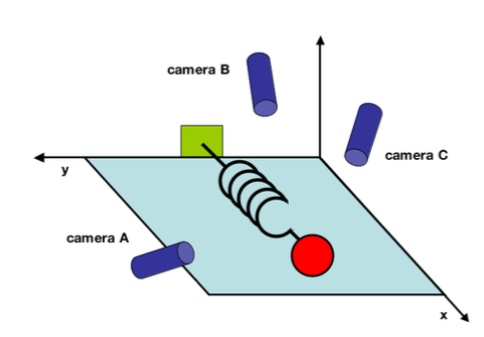
\includegraphics[width=\linewidth]{example}
			\caption{一个实际应用中的例子, 来自\cite{princetonPCA:25:2003}}
			\label{fig:expample}
		\end{figure}
		为了方便理解, 我给出一个实际的情况, 图片参见图\ref{fig:expample}.
		假设我们想研究一个小球的运动状况, 尽管这个小球就在$x$轴上来回运动.
		刚开始研究这个问题的时候, 因为不知道小球在$x$轴方向运动, 所以我们
		在做实验的时候, 就采用了3个摄像头来跟踪小球的轨迹. 
		当我们想要分析这3个摄像头的数据的时候就会十分的困难.
		但是, 可以想见的是: 假如我们碰巧将三个摄像头分别对准了$x, y, z$轴的
		方向. 我们就能分析出问题的关键在$x$轴, 从而我们可以简化我们的数据, 
		因为我们只需要小球在$x$轴上运行的数据就可以了.
		这个改变摄像头方向的过程可以看作代数中的换基的过程.
		即我们希望能够找到一个变换$f$, 使得$Y = f(X)$, 从而得到新的基$Y$,
		且$Y$是那种简化之后的基, 去掉了那些多余的信息.
		
		根据这个观察, PCA在这里做了一个假设: 假设只通过线性变换就能得到一个合理的
		基$Y$. 其实在这里, 不加上这个限制也是可以的, 但是超出了我们的数学水平的范围.

		加上这个假设之后, 原来的式子就可以写成:
		\begin{equation}
			Y = PX
		\end{equation}
		我们把矩阵$P$称作变换矩阵.
		\begin{figure}[ht] \centering
			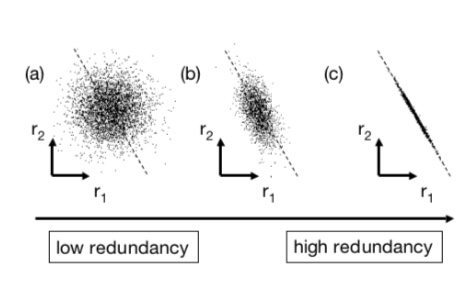
\includegraphics[width=\linewidth]{example1}
			\caption{冗余的量化方式, 来自\cite{princetonPCA:25:2003}}
			\label{fig:example1}
		\end{figure}
		这之后的问题就在于如何找到合适的矩阵$P$来进行基变换.
		那么, 我们要如何评价一个变换矩阵带来的效果呢?
		我们需要首先研究什么是冗余信息.
		参考图\ref{fig:example1}, 假设$r_1, r_2$是我们测量数据中的两个维度.
		图中, 从左到右, 一次给出了这两个维度的相关性的描述. 
		(a)中, 两个维度的数据分布十分的独立.
		而(c)中, 两个维度关系十分明显, 我们可以很容易的使用一个直线方程来表示这些数据.
		对于(c)这种数据, 我们就说, 这两个维度之间, 产生了冗余.
		因为这部分的信息完全可以使用一个维度来表示.
		
		在实际的计算过程中, 我们使用协方差来量化两个维度之间的冗余程度.
		教科书上, 统计量$X, Y$之间的协方差矩阵定义如下:
		\begin{equation}
			cov(X, Y) = \frac{\sum_{i=1}^n(x_i - \bar{x})(y_i - \bar{y})}{n-1}
			\label{eq:cov1}
		\end{equation}
		其中, $x_i$表示了统计量量$X$的第$i$个统计值.
		从(a), 和(c)中, 我们显然可以发现:
		\begin{itemize}
			\item 当两个变量越有相关性的时候, 协方差越大
			\item 当两个变量越不相关的时候, 协方差越小
		\end{itemize}
		这个性质在大二上学期的概率课本中也有相应的讨论.
		从上面的分析中, 我们也可以感受到, 两个变量越相关, 那么他们之间就包含
		了越多的冗余信息. 在PCA中, 协方差自然的被用作了对冗余程度的度量.

		为了方便之后的讨论, 在这里给出协方差的另外一种记法, 可以说, 整个PCA
		都受益与这种特殊的记法. 看到式子\ref{eq:cov1}, 当$\bar{x} = \bar{y} = 0$
		时, 将统计量看作一个向量, 我们可以将上面的协方差写成下面这种形式:
		\begin{equation}
			cov(X, Y) = \frac{XY^T}{n-1}
			\label{eq:cov2}
		\end{equation}
		其中$X = (x_1, x_2, \cdots, x_n), Y = (y_1, y_2 \cdots, y_n)$

		对于一个由统计量构成的矩阵
		\begin{equation}
			X = \left[
				\begin{array}{c}
					x_1 \\
					x_2 \\
					\vdots \\
					x_n
				\end{array}
			\right]
		\end{equation}
		其中$X$的每一行$x_i$都是一个向量, 表示了一个某一个维度的数据,
	   	$X$的每一列则构成了某一次实验的全部数据.
		这样, 将上面的协方差的概念推广, 可以得到$X$的协方差矩阵:
		\begin{equation}
			S_X = \frac{XX^T}{n-1}
		\end{equation}
		对于这个矩阵, 可以得到下面的信息:
		\begin{itemize}
			\item $S_X$是一个实对称矩阵.
			\item $S_X$是一个方阵.
			\item ${S_X}_{i,i}$ 是第$i$维的方差.
			\item ${S_X}_{i,j}(i \not= j)$是第$i$维和第$j$维的协方差.
		\end{itemize}

		回到原来的问题, 显然$Y = PX$中, $X$是我们测量得到的数据, $X$中
		各个统计量之间的协方差可能很大, 但是我们希望能够得到这样的一个
		$P$矩阵, 使得变换之后的$Y$矩阵的不同维度之间的协方差很小.
		即, 希望$Y$的协方差矩阵是一个对角阵.
		\begin{equation}
			\begin{array}{c@{=}c}
				\frac{YY^T}{n-1} & \frac{(PX)(PX)^T}{n-1} \\
				& \frac{P(XX^T)P^T}{n-1} \\
				& P\frac{XX^T}{n-1}P^T \\
				& PS_XP^T
			\end{array}
		\end{equation}
		这样, 我们便确定了转移矩阵$P$具有的性质:$P$是能够使$S_X$对角化的
		矩阵. 这样的矩阵有很多, \cite{princetonPCA:25:2003}中就给出了
		相似对角化, 和SVD两种方法. 

		这里, 因为我在上课的时候并没有怎么听懂SDV, 所以我在实现的时候选择了相似对角化.
		因为$S_X$是一个实对称矩阵, 所以这个矩阵是一定可以对角化的(虽然不能保证每个特征值
		的重数都是1). 根据相似对角化的方法, $P$矩阵就是$S_X$的特征向量构成的矩阵. 且
		\begin{equation}
			PS_XP^T = \left[
				\begin{array}{ccccc}
					\lambda_1 & & & & \\
					          & \lambda_2 & & & \\
							  & & \lambda_3 & & \\
							  & & & \cdots & \\
							  & & & & \lambda_n
				\end{array}
			\right]
		\end{equation}
		其中,$\lambda_i$是$S_X$对应的特征值. 这样, 我们就求得了一个合理的$P$.
		在这里, 即可将$P$中的向量称为主成分.

		更进一步, 为了让结果更加有序, 或者更容易对接之后的处理, 我们一般
		在具体实现的时候, 会在$P$中将特征向量按照对应的特征值, 从大到小排序.
		这样可以保证, 对角化之后的矩阵中, 对角元的值是从大到小变化的.

		上面就是PCA的全部过程. 值得注意的是: 对角化的方法不止一种, 而不同
		的对角化的方法也是有优劣之分的. 在上面讲到的相似对角化的方法中,
		得到的$P$中的每个向量都是特征向量, 他们一般来说都是相互正交的.
		这相当于对于结果多加上了一重条件. 实际上, 在人脸识别的应用中,
		需要使得处于前面的对角元尽量的大, 而处于后面的对角元尽量的小.
		而直接求到的特征向量会正交, 用这样的$P$对角化之后的矩阵
		并不一定比其他的方法对角化得到的矩阵优秀.

	\paragraph{对PCA方法的实际应用}
		在图像分类中, 我们并不是想仅仅求得一个变换. 我们最主要的目的是
		对图片进行降维. 在之前执行PCA的时候, 我们将得到$Y = PX$.
		且我们可以发现, $Y$的协方差矩阵$S_Y$是一个对角矩阵, 每个对角元
		都表示某一个维度的方差. 为了达到降维的目的, 我们必须舍去一些维度,
		不然由于$P$是$\frac{XX^T}{n-1}$的特征向量构成的矩阵, 则$P$和$X$
		的规模是相同的, 也就是最终$Y = PX$是和$X$的形状是相同的.
		就并没有起到降维的目的.
		
		下面来说明, 什么样的维度是可以优先被舍去的. 这里PCA的发明者
		做了一个玄学的假设: 就像上面测量小球的运动轨迹的例子, 
		假设我们有两个摄像头, 摄像头$A$垂直与$x$轴, 摄像头$B$平行$x$轴.
		那么主要的数据应该来自与$A$, 显然$A$中得到的数据的方差要大于$B$
		中的. $B$中数据的方差虽然并不一定完全没有用, 但是更多的时候, 我们可以
		将这些数据作为误差来处理.
		根据对这个例子的理解, 我们可以将方差较小的那些维度舍弃. 
		在用PCA对数据进行降维的时候, 我们总是优先舍弃方差较小的维度.
		这其实就是基于上面的观察而得出的一个假设.

\subsection{一些在实现中遇到的问题}
	\paragraph{计算特征值的效率问题}
		因为数学水平拙劣, 所以我只能采用求特征值的方式对图像做PCA.
		但是假如某个人的图像有10张, 每张$100\times100$. 则$X$
		的规模为$10\times 10000$. 则这个矩阵的协方差矩阵的规模为
		$10000\times 10000$. 对这种规模的矩阵求特征值是我们不能接受的.
		
		我的解决办法是: 先使用重采样, 将原来的图片质量降至$20\times 20$.
		这样人眼还勉强进行识别. 我们可以假装在这个规模的图像还没有丢失
		太多的信息. 然后才对一个$20\times 20$的图像使用PCA来进行最后
		的降维的工作.

		在实际的应用中, 即使对$20\times 20$的像做PCA也仍然不能很好
		的满足应用的要求. 因为当数据库中的人很多的时候, 我们对每一个人
		的相片集, 都需要做一次PCA, 所以还是显得很慢. 所以在实际实现的
		时候, 我在这里做了一个预处理的优化, 即先计算出$P$和均值向量,
		并事先储存在文件之中. 这样在之后的每次查询时, 只需要做一次矩阵
		乘法, 这样就大大降低了运行时间.

	\paragraph{使用最小二乘法的时候矩阵不可逆的问题}
		在使用最小二乘法计算距离的时候, 我们需要使用式\ref{eq:inv}中的求逆运算.
		但是不幸的是, 很多时候$X^TX$都不是满秩的, 这意味着他并不可逆.
		这要求我们在实现的时候需要使用一点技巧. 

		根据上课时老师讲的方法, 我选择了将原来的式\ref{eq:inv}改写为
		\begin{equation}
			\hat{b} = (X^TX + \rho I)^{-1}X^Ty
			\label{eq:fix}
		\end{equation}
		其中$\rho$是一个很小的常数, 我经过一些实验, 发现这个常数适合取到
		$10^{-7}$级别.
		在老师给出的ppt\cite{ShenFuming:ppt}中说明了, 这种改写实际上是执行了
		另外的一种回归---脊回归.
		对于这种回归, 其实际的目标函数其实是:
		\begin{equation}
			\min ||y - \sum_{i=1}^k b_ix_i||^2 + \rho\sum_{i=1}^k b_i^2
			\label{eq:aim}
		\end{equation}
		值得注意的是: 从式\ref{eq:aim}推出式\ref{eq:fix}是比较容易的, 用之前
		的两边求导的方法较容易做到. 但是从式\ref{eq:fix}推出式\ref{eq:aim}
		却很难.

%------------------------------------------------

\section{Results and Discussion}

在本小节中, 我将呈现我所实现的程序在具体的数据集上面的表现, 
并对其进行分析.
\subsection{数据集的选取与测试}
	\paragraph{第一次测试}
		刚刚开始的时候, 我使用了AT\&T的人脸识别数据集\cite{database}.
		但是我不太清楚业内具体是如何使用这种数据的. 所以我采用了一种比较
		简单的测试方法. 

		具体的方法是: 每次从一个人的照片集中取出一张照片(从照片集中删掉),
		然后将这个图片作为程序的输入, 看程序是否能够得到原来那个人的名字.
		统计成功的次数. 然后就能用来判断程序的. 然后我通过不停的调整参数
		(e.g. 调整PCA降维之后保留的维数), 通过一波面向数据编程, 使得
		识别率达到了喜人的97\%.

	\paragraph{第二次测试}
		这一次测试我采用了老师放在网盘上的各个同学提供的自拍照作为测试的
		数据集. 这一次的测试成绩并没有之前使用标准数据集测试得到的数据来得好.
		但是这主要是因为很多同学并没有理解人脸识别的意思, 人脸识别,
		并不包括人脸检测, 但是很多同学给的相片却是半身照, 这大大影响了识别的
		准确率.

	\paragraph{关于运行速度}
		经过测试, 预处理之后, 我的程序只需要300ms左右就可以完成一个人脸的识别.
		并且, 虽然我没有具体实现, 在使用了PCA降维过后, 整个数据库所需的储存空间
		是会大大降低的, 原来百万维的图片, 经过两步降维之后, 变成了一个
		50维以内的向量. 这不仅节约了磁盘的空间, 而且降低了程序运行时的IO开销.

%------------------------------------------------
\phantomsection
\section*{Acknowledgments} % The \section*{} command stops section numbering
\addcontentsline{toc}{section}{Acknowledgments} % Adds this section to the table of contents
在实现这个程序的时候, 实际上最开始参考的是\cite{tutorial:PCA}
这篇文章, 但是就像这篇文章的名字那样, 写得太浅了, 导致我并没有真正
搞懂PCA的内部原理.

本文中出现的最小二乘法, 实际是在概率论\cite{prob}中讨论多元线性回归的时候提到的.


%----------------------------------------------------------------------------------------
%	REFERENCE LIST
%----------------------------------------------------------------------------------------
\phantomsection
\bibliographystyle{unsrt}
\bibliography{sample}

%----------------------------------------------------------------------------------------

\phantomsection
\section*{Appendix}
\addcontentsline{toc}{section}{Appendix} % Adds this section to the table of contents
为了使得这篇文章显得更加的丰满, 我将我的实现过程贴到这篇附录当中.
只是字可能稍微有点小, 不过反正都是电子版.

\setmainfont{Monaco} % fonts
\subsection*{face\_ver2.py}

\begin{lstlisting}[language=python]
#这个文件是程序的入口
#python 库
import sys
import os
import pickle

#scipy 库
from PIL import Image
import numpy as np
from scipy import linalg

#本地库
import PrincipalComponentsAnalisis as pca
import LinearRegression as linreg

def classify(sample, dataBase, distance):
    """
    int classify(sample, dataBase, simpFunc, distance)
    用于判断sample到底归属于dataBase中的哪一个类别
    sample 和 dataBase 中的数据都已经降维
    输入:
        sample : numpy.ndarray
        dataBase : [numpy.ndarray] (注意到这个数据的外层套了一个list)
        其中dataBase中的每一个ndarray表示了一个空间的基
        distance : 距离函数(用于求sample到每个空间的距离)
    输出:
        返回一个整数, 表示sampleOri属于的那个dataBaseOri项的编号
    """
    dis = []
    for i in range(len(dataBase)):
        dis.append(distance(sample, dataBase[i]))
    minx, minWhere = dis[0], 0 
    l = len(dis)
    for i in range(l):
        if dis[i] < minx:
            minx, minWhere = dis[i], i
    return minWhere

def getPicture(Dir):
    """
    输入:
        一幅图的位置
    输出:
        一个灰度矩阵(1 x n)
        内部值为float64
        且归一化
    """
    data = Image.open(Dir)
    data = data.resize((20, 20)) #调整图片的大小
    data = np.asarray(data)
    data = data.astype('float64') #将所有输入的图片都转化为float64类型
    if len(data.shape) == 3: #这说明这个是一张彩图
        data = data[:, :, 0] + data[:, :, 1] + data[:, :, 2] / 3.0
    data.reshape([1, data.size])
    data = data / linalg.norm(data) #归一化
    return data.reshape([1, data.size])

def readPerson(Dir):
    """
    用于读取某个人的全部的数据集
    输入:
        Dir : 数据集目录 (str)
    输出:
        一个人的照片矩阵
        其中每一个照片为矩阵的一行
    """
    files = os.listdir(Dir)
    dirs = [Dir + '/' + File for File in files if File[0] != '.']
    faces = getPicture(dirs[0])
    l = len(dirs)
    for i in range(1, l):
        tmpFace = getPicture(dirs[i])
        faces = np.append(faces, tmpFace, axis = 0)
    return faces

def genPersonDir(dataBaseWhere):
    """
    用于生成dataBaseWhere的下级目录
    """
    names = os.listdir(dataBaseWhere) #读取数据库中的文件夹的名字
    names = [item for item in names if item[0] != '.'] #注意去掉隐藏文件
    names.sort();
    dirs = [dataBaseWhere + '/' + name for name in names]
    return names, dirs


def learningAllPerson(dataBaseWhere, simplify, fresh = False):
    """
    输入: 
        dataBaseWhere : dataBase位置(目录)
        simplify : 降维函数
        fresh : 是否需要更新之前的学习数据
    输出:
        无
    功能:
        生成一个转移矩阵, 存放在dataBaseWhere/.info中
        为每个人的照片集生成一个已经降维的矩阵, 存放在dataBaseWhere/Person/.info中
    """
    if os.path.exists(dataBaseWhere + '/' + '.info') and (not fresh):
        return

    dirs = genPersonDir(dataBaseWhere)[1]

    data = readPerson(dirs[0])
    for i in range(1, len(dirs)):
        data = np.append(data, readPerson(dirs[i]), axis = 0)

    output = open(dataBaseWhere + '/' + '.info', 'wb')
    simpFunc = simplify(data, data.shape[1], 40, data.shape[0], mode = 'func')
    pickle.dump(simpFunc, output)
    output.close()

    func = pca.genTrans(simpFunc)
    for Dir in dirs:
        curDir = Dir + '/' + '.info'
        output = open(curDir, 'wb')
        pickle.dump(func(readPerson(Dir)), output)
        output.close()



def recognizeFace(faceWhere, dataBaseWhere, distance):
    """
    输入: 
        faceWhere : 样本位置(文件)
        dataBaseWhere : dataBase位置(目录)
        保证dataBaseWhere中存放了各个不同的人的文件夹
        |-dataBaseWhere
            |-Person 1
            |-Person 2
            |-Person 3
            |...
            |-Person n
        distance : 距离函数
    输出:
        样本属于的人的名字(dataBaseWhere中文件夹名)
    """
    face = getPicture(faceWhere)
    names, dirs = genPersonDir(dataBaseWhere)

    dataBase = []
    for Dir in dirs:
        info = open(Dir + '/' + '.info', 'rb')
        dataBase.append(pickle.load(info))
        info.close()

    info = open(dataBaseWhere + '/' + '.info', 'rb')
    simpFunc = pca.genTrans(pickle.load(info))
    info.close()

    ID = classify(simpFunc(face), dataBase, distance)

    return names[ID]

if __name__ == '__main__' : #程序入口
    fs = False
    if len(sys.argv) >= 4 and sys.argv[3] == 'fresh':
        fs = True
    learningAllPerson(sys.argv[1], pca.PCA, fresh = fs)
    ans = recognizeFace(sys.argv[2], sys.argv[1], linreg.linearRegression)
    print (ans)
\end{lstlisting}

\subsection*{PrincipalComponentsAnalisis.py}
\begin{lstlisting}[language=python]
#本文件主要用于实现PCA, 用于对输入图片的降维
import numpy as np
from scipy import linalg

class eigPair(object):
    """
    用于储存特征值与特征向量的有序对, 构造比较函数
    最终参与排序
    """
    def __init__ (self, val, vec):
        """
        val : float64
        vec : numpy.array
        """
        self.val = abs(val) #需要按照绝对值的大小排序
        self.vec = vec
    def __lt__ (self, other):
        return self.val > other.val #按降序排列
    def __str__ (self): #用于调试输出
        return '[{}, {}]'.format(self.val, self.vec.__str__())

def PCA(data, inputCntDim, outputCntDim, cntVec, mode = 'ans'):
    """
    这个函数用于提供计算PCA的功能.
    输入: 
        data: 用于进行PCA处理的数据(二维矩阵)         (np.array)
        inputCntDim: 输入数据data中待处理的数据的维数 (int)
        outputCntDim: 输出数据中希望保留的维数        (int)
        cntVec: data中包含的独立的向量的个数          (int)
        mode: 希望得到的解的形式
              'ans' : 直接返回答案
              'func' : 返回转移矩阵
    输入矩阵的形式:
        /  x[1][1]         x[1][2]      ...    x[1][inputCntDim]    \\
        |  x[2][1]         x[2][2]      ...    x[2][inputCntDim]     |
        |    ...             ...        ...       ...                |
        \\x[cntVec][1]    x[cntVec][2]  ...   x[cntVec][inputCntDim] /
        <=>
        / Img[1]     \\
        | Img[2]     |
        |  ...       |
        \\Img[cntVec]/
        具体实现时从0开始编号
    输出:
        一个矩阵, 包含和data相同的行数, 列数变为outputCntDim, 丢失尽量少测信息
    """
    data.dtype = 'float64' #确认类型
    #计算并剪去平均数
    mean = np.mean(data, axis = 0)
    for i in range(cntVec):
        data[i, :] -= mean

    #计算相关系数
    cov = np.cov(data, rowvar = False)
    
    #计算特征值与特征向量并排序
    eigenvalue, eigenvector = linalg.eig(cov)
    eigList = [eigPair(eigenvalue[i], eigenvector[:, i]) for i in range(inputCntDim)]
    eigList.sort()

    #选择前面outputCntDim个特征向量
    featureVec = eigList[0].vec
    for i in range(1, outputCntDim):
        featureVec = np.append(featureVec, eigList[i].vec)
    featureVec = featureVec.reshape([outputCntDim, inputCntDim]) #调整形状

    #得到PCA之后的结果
    def trans(data):
        return featureVec.dot(data.transpose()).transpose()

    if mode == 'ans': 
        return trans(data)
    elif mode == 'func':
        return featureVec, mean

def genTrans(func):
    def trans(data):
        for i in range(data.shape[0]):
            data[i, :] -= func[1]
        return func[0].dot(data.transpose()).transpose()
    return trans

if __name__ == '__main__': #用于测试
    data = np.array([[2.5, 2.4],
                     [0.5, 0.7],
                     [2.2, 2.9],
                     [1.9, 2.2],
                     [3.1, 3.0],
                     [2.3, 2.7],
                     [2.0, 1.6],
                     [1.0, 1.1],
                     [1.5, 1.6],
                     [1.1, 0.9]])
                     
    ans = PCA(data.copy(), data.shape[1], 1, data.shape[0], mode = 'func')
    func = genTrans(ans)
    ans = func(data)
    print(ans)
\end{lstlisting}

\subsection*{LinearRegression.py}
\begin{lstlisting}[language=python]
#这个文件用于实现用多元线性回归

import numpy as np
from scipy import linalg

def linearRegression(y, X):
    """
    输入:
        y : numpy.ndarray
        X : numpy.ndarray
        需要保证y和A的列数相同(按照行向量的方式储存)
        y和A中的每一个行向量都是一张素材
    """
    rho = 0.005
    dim = X.shape
    b = linalg.inv(X.dot( X.transpose() ) + np.identity(dim[0]) * rho).dot(X.dot( y.transpose() )) #加了一个单位矩阵, 保证可逆
    yPre = X.transpose().dot(b)
    dy = y.transpose() - yPre
    return linalg.norm(dy.transpose().dot(dy)+ rho * b.transpose().dot(b))

if __name__ == '__main__' : #测试
    y = np.array([[15.8, 16.0, 15.9, 16.2, 16.5, 16.3, 16.8, 17.4, 17.2]])
    A = np.array([[0, 1, 0, 1, 2, 0, 2, 3, 1],
                  [0, 0, 1, 1, 0, 2, 2, 1, 3]])
    linearRegression(y, A)
\end{lstlisting}

\end{document}
